\documentclass[tikz,border=3pt]{standalone}
\usepackage{amsmath}
\usetikzlibrary{arrows.meta,positioning,calc}
\definecolor{navy}{HTML}{153B5B}
\definecolor{blue}{HTML}{2D6A9F}
\definecolor{teal}{HTML}{2A9D8F}
\definecolor{gold}{HTML}{E9A23B}
\definecolor{ink}{HTML}{24313A}
\definecolor{pale}{HTML}{F4F7F9}
\tikzset{
  box/.style={draw=navy,line width=.8pt,rounded corners=2pt,fill=pale,
    minimum height=9mm,align=center,font=\sffamily\small,inner xsep=5pt},
  arrow/.style={-{Latex[length=2.2mm]},line width=.8pt,draw=ink},
  label/.style={font=\sffamily\scriptsize,text=ink}
}
\begin{document}
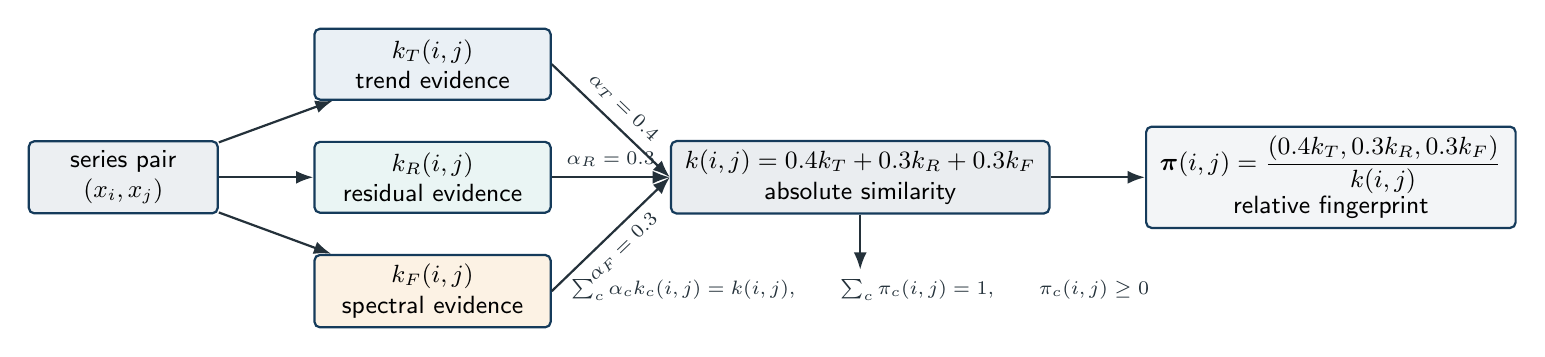
\begin{tikzpicture}[node distance=5mm and 8mm]
  \node[box,minimum width=24mm,fill=navy!8] (pair) {series pair\\$(x_i,x_j)$};
  \node[box,above right=5mm and 12mm of pair,minimum width=30mm,fill=blue!10] (kt)
    {$k_T(i,j)$\\trend evidence};
  \node[box,right=12mm of pair,minimum width=30mm,fill=teal!10] (kr)
    {$k_R(i,j)$\\residual evidence};
  \node[box,below right=5mm and 12mm of pair,minimum width=30mm,fill=gold!14] (kf)
    {$k_F(i,j)$\\spectral evidence};

  \node[box,right=15mm of kr,minimum width=36mm,fill=navy!9] (sum)
    {$k(i,j)=0.4k_T+0.3k_R+0.3k_F$\\absolute similarity};
  \node[box,right=12mm of sum,minimum width=38mm,fill=navy!5] (fp)
    {$\boldsymbol\pi(i,j)=
      \dfrac{(0.4k_T,0.3k_R,0.3k_F)}{k(i,j)}$\\relative fingerprint};

  \draw[arrow] (pair) -- (kt);
  \draw[arrow] (pair) -- (kr);
  \draw[arrow] (pair) -- (kf);
  \draw[arrow] (kt.east) -- node[label,above,sloped] {$\alpha_T=0.4$} (sum.west);
  \draw[arrow] (kr.east) -- node[label,above] {$\alpha_R=0.3$} (sum.west);
  \draw[arrow] (kf.east) -- node[label,below,sloped] {$\alpha_F=0.3$} (sum.west);
  \draw[arrow] (sum) -- (fp);

  \node[label,below=7mm of sum] (identity)
    {$\sum_c \alpha_c k_c(i,j)=k(i,j),\qquad
      \sum_c\pi_c(i,j)=1,\qquad \pi_c(i,j)\geq0$};
  \draw[arrow] (sum.south) -- (identity.north);
\end{tikzpicture}
\end{document}

